\chapter{Cài đặt}
\label{Chapter2}

\section{Data source}

Theo tài liệu của thư viện Transformers, tóm tắt có thể được mô tả là việc tạo ra một phiên bản ngắn hơn của một tài liệu hoặc một bài báo mà vẫn nắm bắt được tất cả các thông tin quan trọng.

Trong trường hợp này, chúng ta sẽ tóm tắt các cuộc hội thoại bằng cách sử dụng một tập dữ liệu chứa các đoạn chat.

Đối với nhiệm vụ này, chúng ta sẽ sử dụng Tập dữ liệu SamSum, bao gồm ba tệp csv cho huấn luyện, kiểm tra và xác thực. Tất cả các tệp này được cấu trúc thành một id cụ thể, một cuộc hội thoại(a dialogue) và một bản tóm tắt( a summary). Tập dữ liệu SamSum bao gồm các đoạn chat, lý tưởng cho việc tóm tắt các cuộc hội thoại.\\

\lstinputlisting[language=Python]{SourceCode/data.py}

\section{Thư viện}

\lstinputlisting[language=Python]{SourceCode/importlibrary.py}

\section{Chưa rõ}

\lstinputlisting[language=Python]{SourceCode/unknow.py}

\section{Tập dữ liệu}

Chúng ta có thể bắt đầu phân tích tập dữ liệu bằng cách tải tất cả ba tập dữ liệu có sẵn, bao gồm tập huấn luyện (train), tập kiểm tra (test) và tập xác thực (val).\\

\lstinputlisting[language=Python]{SourceCode/explore.py}

\begin{figure*}[htp]
    \centering
    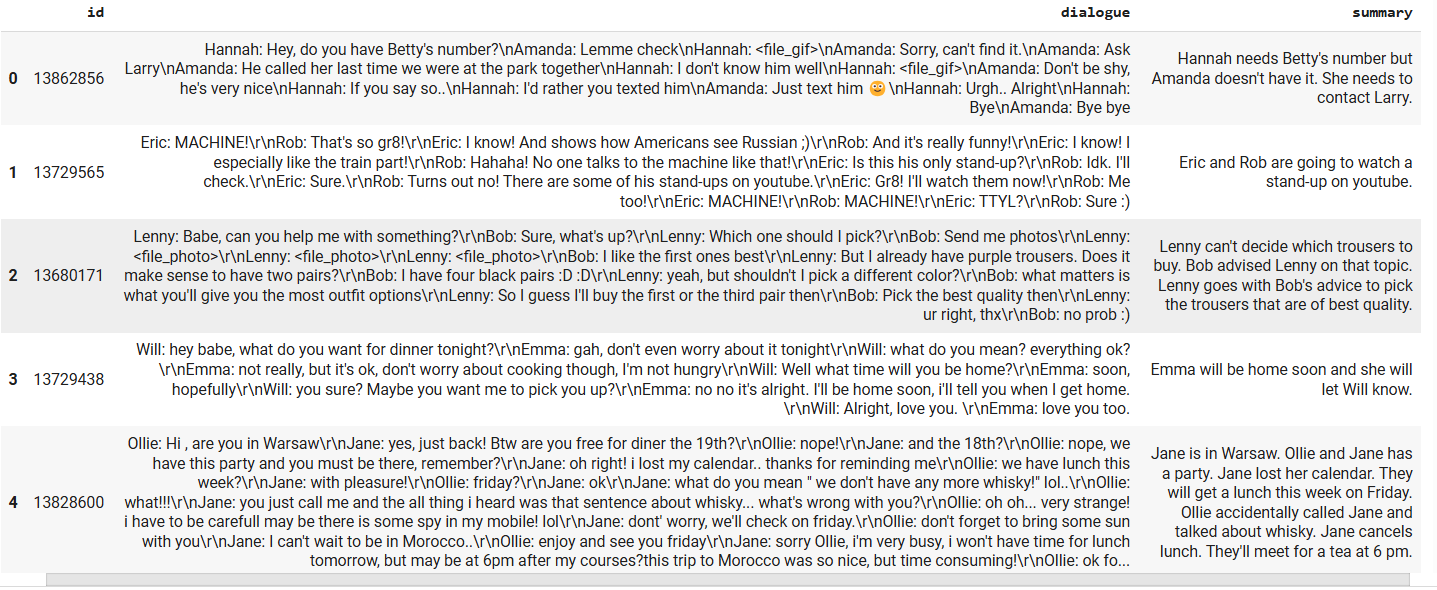
\includegraphics[scale=.5]{images/df.png}
    \caption{Minh họa Dataframe}
    \end{figure*}
\pagebreak

